The normalized chimera-like index of the entire physical region is shown in \cref{fig:aphysical_chimera}.
Near the maximal edge of the physical region, the highest values of the chimera index appear to follow a slope of $-1$.
It is unsurprising that chimera states would be prevalent when the coupling is large (out near the boundary of the aphysical range).

What is surprising, however, is the presence of the chimeric patch in the bottom left corner of \cref{fig:aphysical_chimera}, shown at a higher resolution in \cref{fig:zoom_chimera}.
\begin{figure}[ht]
  \centering
  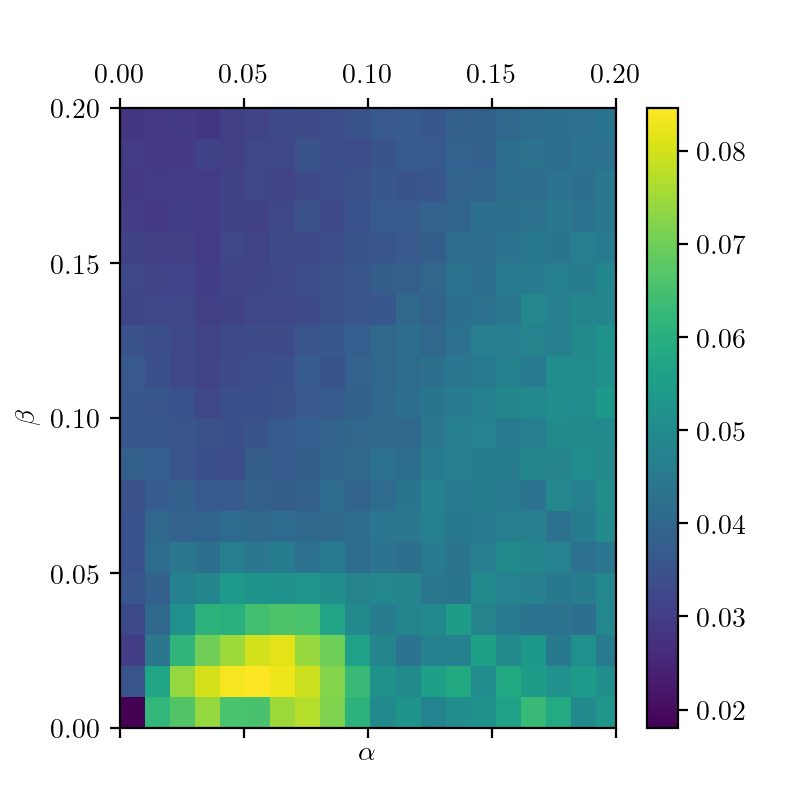
\includegraphics{figure/zoom_chimera}
  \caption[Zoomed landscape]{The chimera index of runs with $(\hra, \hrb) \in (0, 0.2) \times (0, 0.1)$.
    As before, the chimera-like index is normalized to $\frac{1}{7}$.
    Note that the values of the index are much higher in this patch than in most of the rest of $(\hra, \hrb) \in (0, 0.9) \times (0, 0.9)$ (\cref{fig:aphysical_chimera}).
    The dashed line shows $\beta = \alpha$.
  }
  \label{fig:zoom_chimera}
\end{figure}
Plotting the results of the simulations (\cref{fig:mean_058_010,fig:overhead_058_010}),
it is evident that this is not a calculation error, but is an actual feature of the parameter landscape.
\begin{figure}[ht]
  \centering
  \begin{subfigure}{\textwidth}
    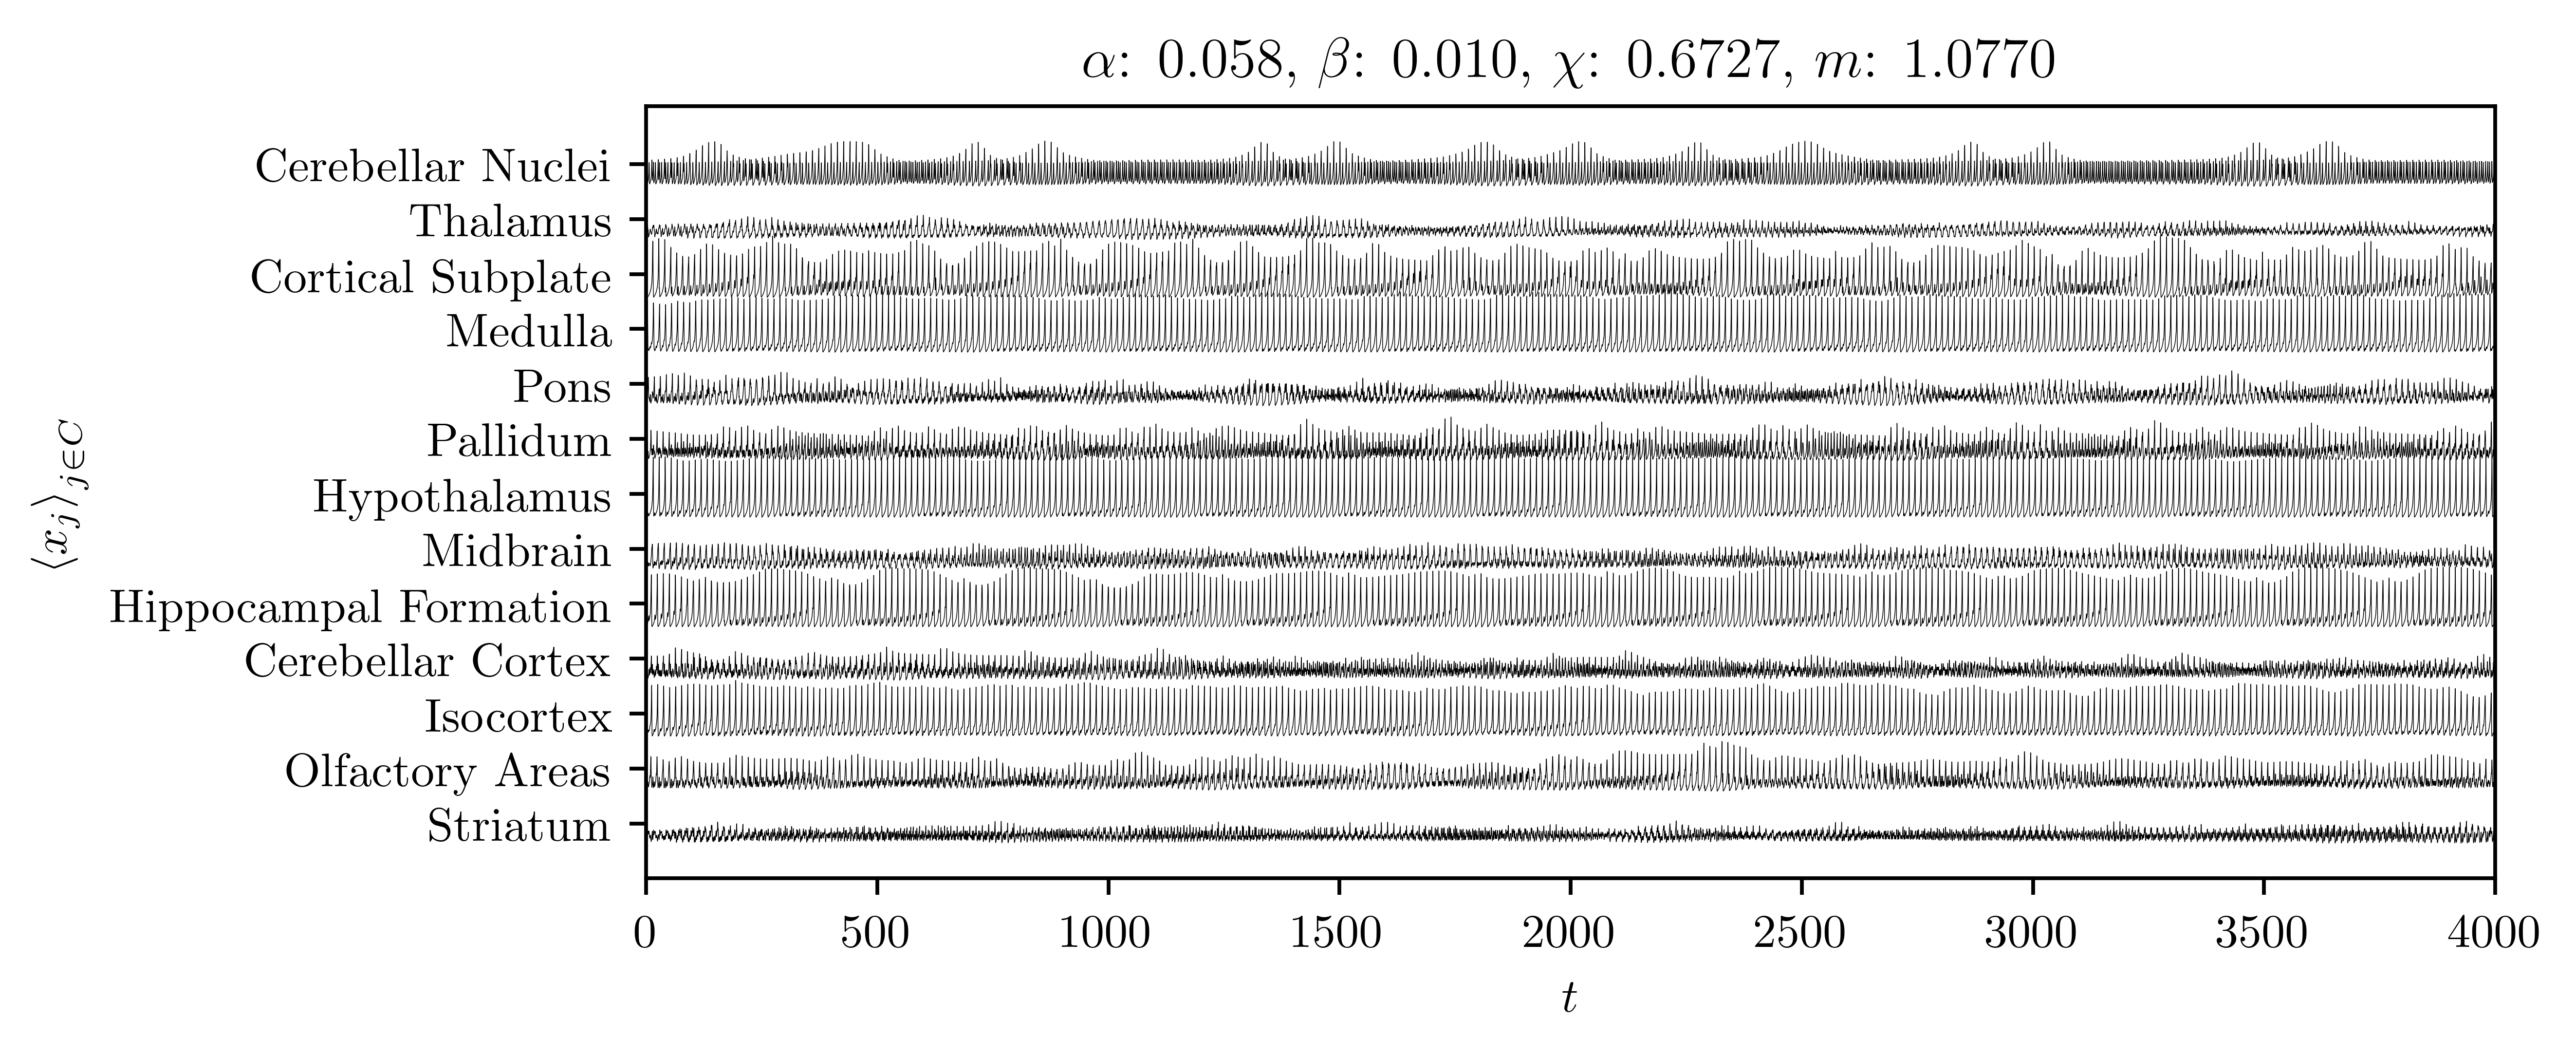
\includegraphics[width=\textwidth]{figure/means-0_058-0_010}
    \caption{}
    \label{fig:mean_058_010}
  \end{subfigure}
  \begin{subfigure}{\textwidth}
    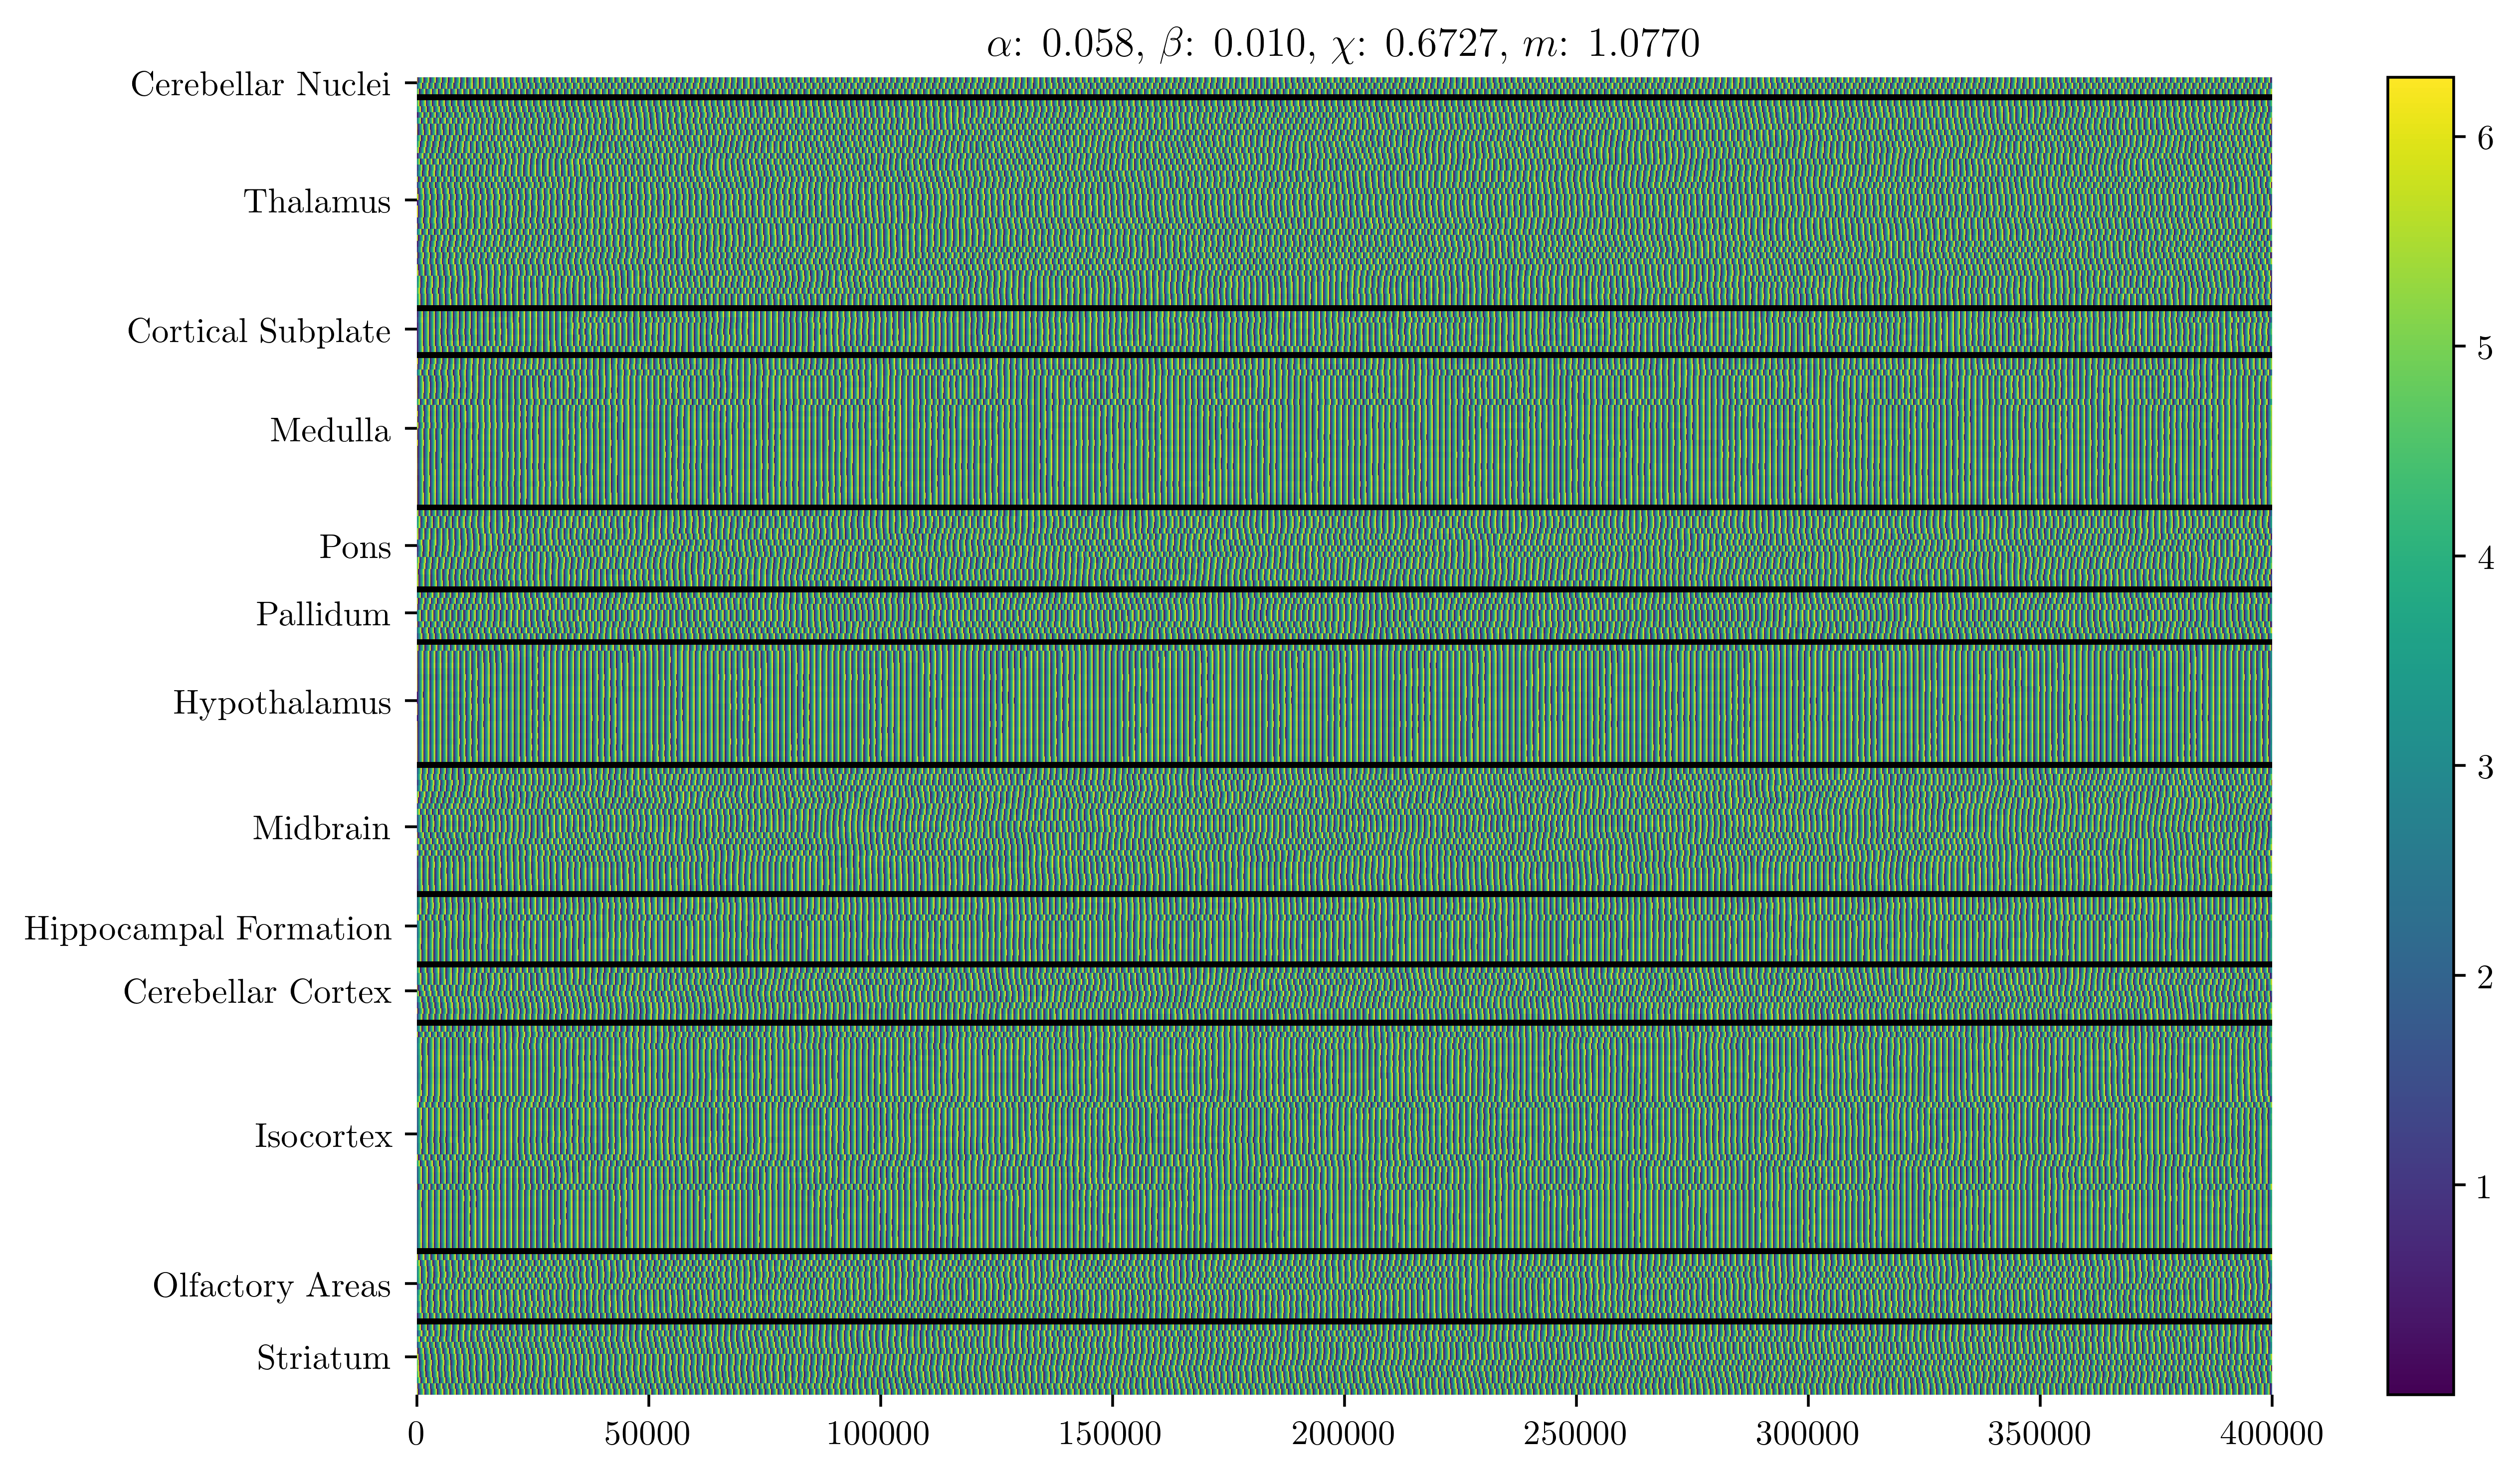
\includegraphics[width=\textwidth]{figure/overhead-0_058-0_010}
    \caption{}
    \label{fig:overhead_058_010}
  \end{subfigure}
  \caption[Highly chimeric simulation]{A run of the Hindmarsh-Rose simulation in the chimeric island.
    (a) The mean membrane potential within each cortex.
    (b) The phase $\phase$ of the entire timeseries for a simulation of the Hindmarsh-Rose network.
    Synchronization is most consistently evident in the medulla, the hypothalamus, and the isocortex.
  }
  \label{fig:058_010}
\end{figure}

The highly chimeric portion of the landscape appears to be mostly below the $\beta = \alpha$ line.
This is reasonable, as chimera states occur when coupling within groups is greater than coupling between groups.
A small portion of the chimeric patch lies above the $\beta = \alpha$ line, likely due to the fact that the average strength between cortices is greater than the average strength within cortices (see \cref{fig:g_over_n}).

$\chimera$ greatly lessens at $\alpha \approx 0.1$.
A possible explanation for this comes from comparing the order of $\dot{\hrx}$ without the coupling terms, and the coupling terms themselves.
From our simulation, we find that $\dot{\hrx}$ without the coupling terms ranges roughly from -6 to 3.
The coupling terms each\footnote{Since the same can be said for both $\alpha$ and $\beta$, we will discuss only $\alpha$, with the understanding that $\beta$ could be substituted into the proceeding sentences.} range from 0 to approximately $30 \alpha$.
That means that, when $\alpha > 0.1$, the coupling is at least of the same order as the sum of the rest of the terms in the equation.
This leads to a qualitative difference between the two states, which likely manifests itself as the less chimeric states.

%%% Local Variables:
%%% mode: latex
%%% TeX-master: "../../main"
%%% End:
